% !TEX root=../../Thesis.tex
\newcommand {\matr}[2]{\left[\begin{array}{#1}#2\end{array}\right]}
\newcommand{\E}{\mathbb{E}}
\newcommand{\tr}{\mathrm{tr}}
\newcommand{\x}{{\mathbf{x}}}
\renewcommand{\u}{{\mathbf{u}}}
\newcommand{\w}{{\mathbf{w}}}
\renewcommand{\r}{{\mathbf{r}}}

\chapter{Modeling Intersection Driving Scenarios}
\label{ch:modeling_intersection}
\tommy{modeling is the key to...}
\begin{center}
  \textit{\textbf{RQ 1: How can \gls{rl} be used to create a decision-making agent for driving through intersections?}}
\end{center}
  \vspace{12pt}
  
Driving through an intersection is a sequential decision-making problem and can be mathematically formulated using a \gls{mdp}, introduced in Section~\ref{sec:background_mdp}. As mentioned in the introduction, this thesis will focus on driving in intersections together with other drivers and not only follow the traffic rules but also be able to adapt to other drivers intentions. Since the intention of other drivers is not observable with any existing sensors today, \gls{pomdp} is better suited to formulate the problem. 

Modeling the intersection problem in a good way is the key to finding a good decision-making policy. This chapter highlights the key points of the \gls{pomdp} for the intersection problem in this thesis. The state space, action space, 
 


\Citet{Shalev2016} raises two concerns when using Machine learning, specially Reinforcement learning, for autonomous driving applications: ensuring functional safety of the Driving Policy and that the Markov Decision Process model is problematic, because of unpredictable behavior of other drivers.
In the real world, intentions of other drivers are not always deterministic or predefined. Depending on their intention, different actions can be chosen to give the most comfortable and safe passage through an intersection.
They also noted that in the context of autonomous driving, the dynamics of vehicles is Markovian but the behavior of other road users may not necessarily be Markovian.

This Chapter defines the \gls{pomdp} for the intersection studied in this thesis. 

% \section{Intersection scenarios}

% % \begin{figure}
% % \centering
% % \begin{tikzpicture}

% % 	% Crossing
% % 	\def\crosstopy{8}
% % 	\def\crossboty{-2.5}
% % 	\def\crossleftx{-7}
	
% % 	\draw[thick] (\crossleftx, 1) -- (-1, 1) -- (-1, \crosstopy);
% % 	\draw[thick] (\crossleftx, -1) -- (-1, -1) -- (-1, \crossboty);
% % 	\draw[thick] (1, \crosstopy) -- (1, 1) -- (3, 1);
% % 	\draw[thick] (1, \crossboty) -- (1, -1) -- (3, -1);
	
% % 	cars
% % 	\node[inner sep=0pt] (ego_car) at (-6,0)
% % 	{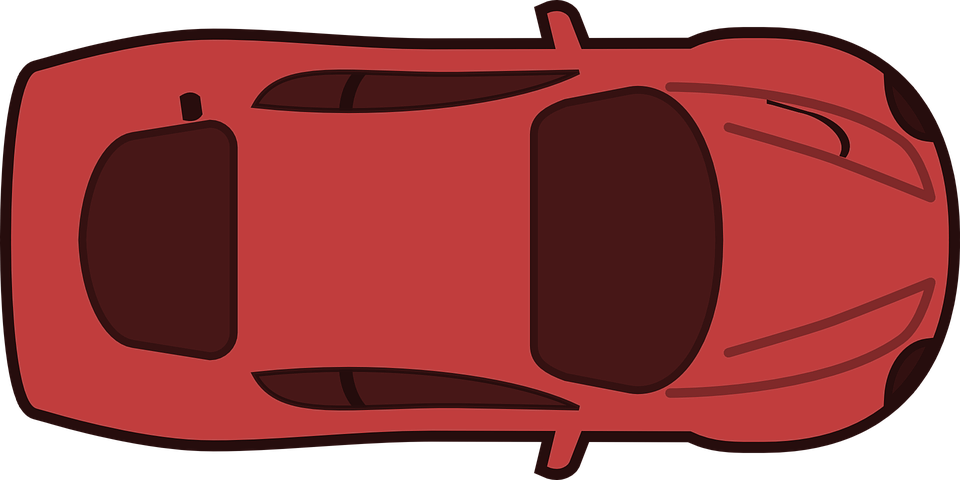
\includegraphics[width=.18\textwidth, angle=0]{figures/ego_car_top_down.png}};
% % 	\draw[->] ([yshift=0.2cm]ego_car.east) -- node[above] {$v^{ego}$} ($ (ego_car) + (2,0.2)$ );
% % 	\draw[|-|] ([yshift=-0.2cm]ego_car.east) -- node[below] {$p^{ego}_{0}=v^{ego}*\tau_{int}$} (-1,-0.2);

% % 	\node[inner sep=0pt] (target_car_3) at (0,7)
% % 	{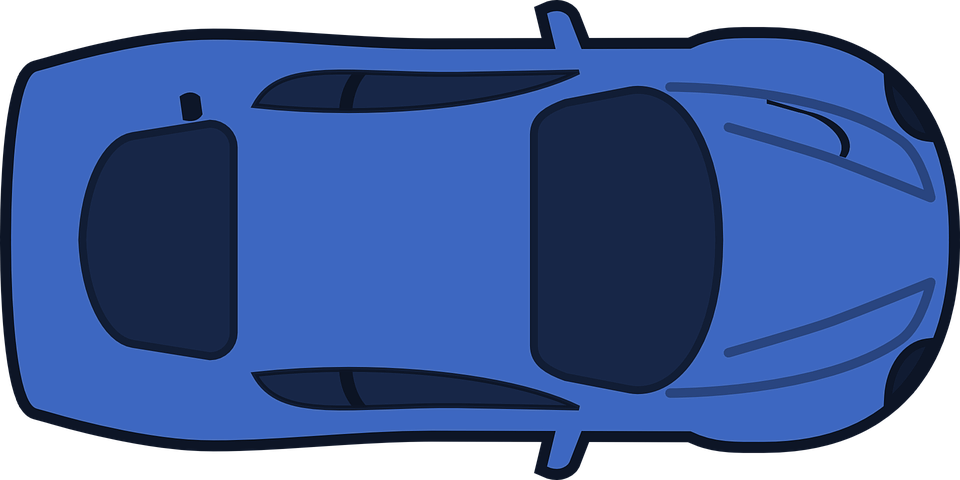
\includegraphics[width=.18\textwidth, angle=-90]{figures/target_car_top_down.png}};
% % 	\node (tc_text3a) [right=of target_car_3, align=center] {Car 3};
% % 	\node (tc_text3b) [left=of target_car_3, align=center] {Conflict Car};
% % 	\draw[->] ([xshift=0.3cm]target_car_3.south) -- node[right] {$v^{3}_0$} ($ (target_car_3) + (.3,-2)$ );
% % 	\draw[|-|] ([xshift=-0.8cm]target_car_3.south) -- (-.8,1);
% % 	\node (tc_tti) [below left= 0.9cm and -0.7cm of target_car_3, align=center] {$p^3_{0}$  \\ $\tau_{int}$};

% % 	\node[inner sep=0pt] (target_car_2) at (0,2.5)
% % 	{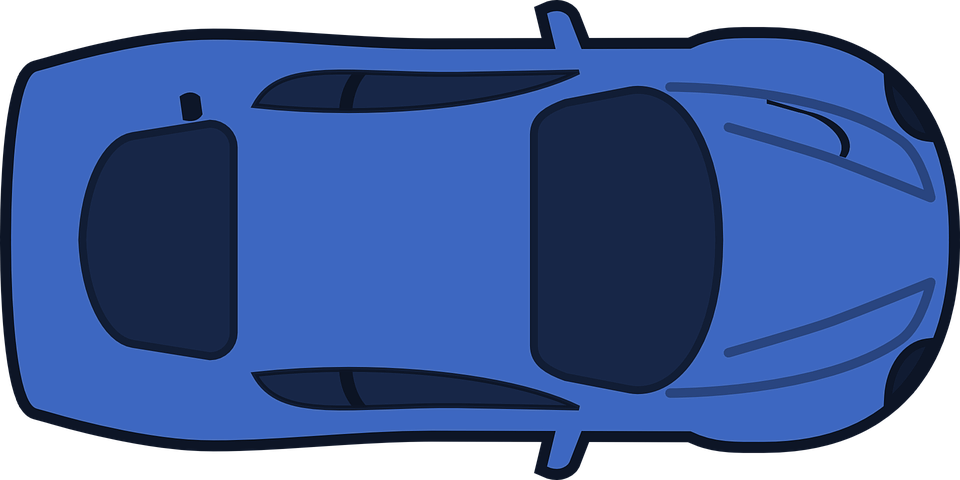
\includegraphics[width=.18\textwidth, angle=-90]{figures/target_car_top_down.png}};
% % 	\node (tc_text2) [right=of target_car_2] {Car 2};
	
% % 	\node[inner sep=0pt] (target_car_1) at (0,-1.5)
% % 	{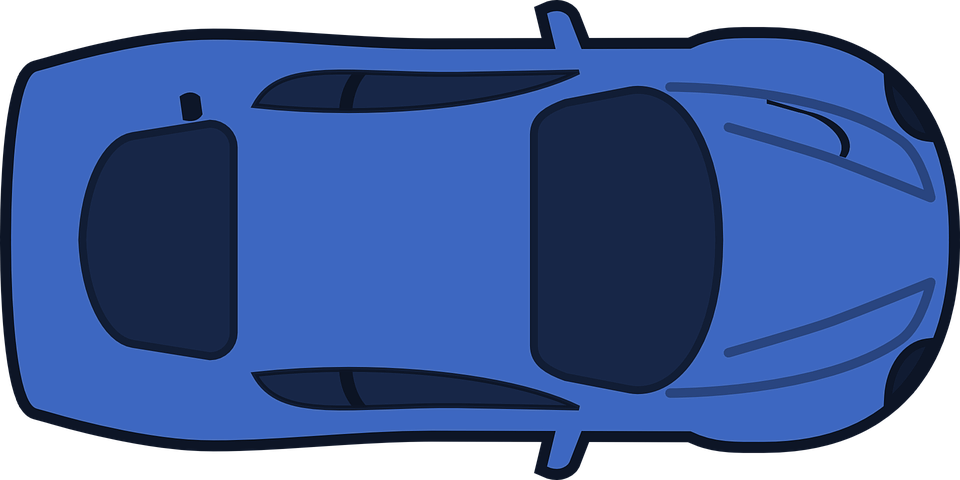
\includegraphics[width=.18\textwidth, angle=-90]{figures/target_car_top_down.png}};
% % 	\node (tc_text1) [right=of target_car_1] {Car 1};

% % \end{tikzpicture}
% % \caption{Observations that makes the state}
% % \label{fig:intersection_scenario}
% % \end{figure}

% \begin{figure}
% \centering
% \begin{tikzpicture}
% 	\def\xstart{-7};

% 	% Crossing
% 	\draw[line width=0.5mm] (\xstart, 1) -- (-1, 1) -- (-1, 5);
% 	\draw[line width=0.5mm] (\xstart, -1) -- (-1, -1) -- (-1, -2);
% 	\draw[line width=0.5mm] (1, 5) -- (1, 1) -- (3, 1);
% 	\draw[line width=0.5mm] (1, -2) -- (1, -1) -- (3, -1);
	
% 	% cars
% 	\node[inner sep=0pt] (ego_car) at (-6,0)
% 	{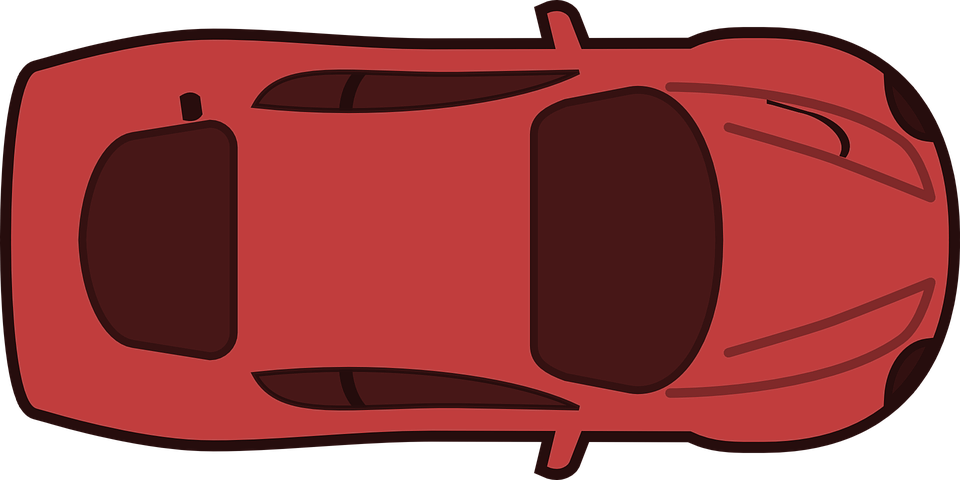
\includegraphics[width=.18\textwidth, angle=0]{figures/ego_car_top_down.png}};
% 	\node[inner sep=0pt] (target_car) at (0,4)
% 	{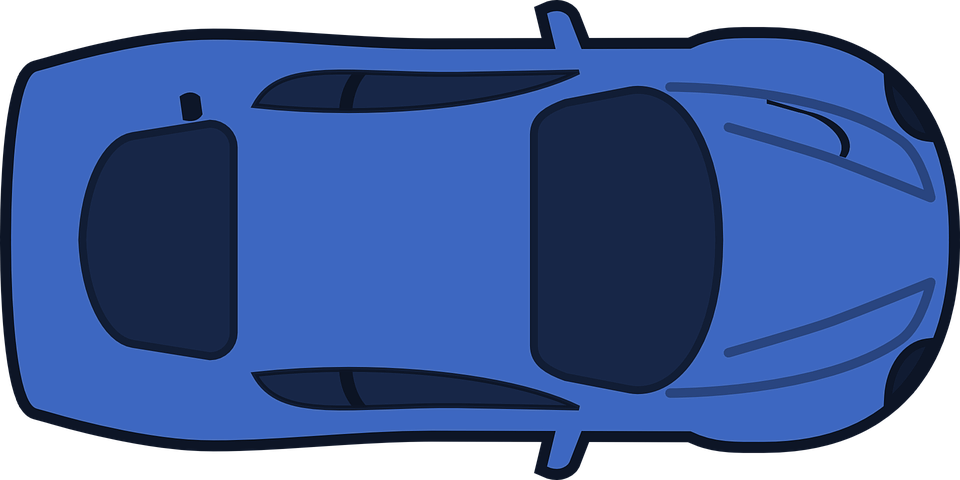
\includegraphics[width=.18\textwidth, angle=-90]{figures/target_car_top_down.png}};

% \end{tikzpicture}
% \caption{}
% \label{fig:intersection_scenario}
% \end{figure}


% Figure \ref{fig:intersection_scenario} shows a simple intersection with one crossing point. 
% \tommy{show examples of intersections.}
% \tommy{zone 0 - after intersection, zone 1 - conflict zone, zone 2 - right before the intersection, zone 3 - first obsereved interstion to zone 2}

\section{State space}
From Section~\ref{sec:background_mdp}, the state space contains all the information necessary about the agent and environment to be able to transition to any given state. In the scenario from Figure~\ref{fig:intersection_scenario}, the red car on the horizontal lane represents the ego vehicle and the blue cars on the vertical lane are the other vehicels. 
Let's start by defining the information needed. Starting with the terminal states: goal, to know if ego vehicles has crossed the intersection and reached the goal. The distance from ego to goal $p_{goal}$ is needed. For collision, the position of all surrounding traffic participants and a description of the intersection itself is necessary. Instead of using a Cartesian coordinate system, I propose using relative distance measures instead. This way, states describing the intersection and its participants are generalizable to different intersection designs, e.g., the angle of incidence and number of crossing points. 
Then, the velocity and acceleration of all the traffic participants is necessary to be able to predict what position they will be in the next state. Finally, the intention of all the other participants. This state is necessary to efficently navigate through an interdection. \paperBelief shows a comparision between two fully observable \gls{mdp}s, one with intention and the other one without and the results show that having an intention state reduce number of collisions. 
\paperLSTM proposed the first set of states. %The states describing ego and other vehicle are spearated. Repeat the states for each other vehicle we observe. 
\tommy{Coordinate system, distances to intersection, position, velocity and accelration of other vehicles. abstract away the information about traffic lights, traffic signs, as intention}

\section{Action space}
\tommy{options, take way, give way, follow car}
One of the limitations of deep Q-learning is that the action space has to be discreet. In other work it is common to set the action space to diffecnt acceleration request. However, I propose using short term goals as actions. The short term goals are high level objectives like stop at the start of the intersection, follow car with id 1 or drive through the intersection at the reference speed. 
This high level action is then sent to a sliding mode controller that generates an acceleration. 
In \paperMPC the actions is sent to a \gls{mpc} to generate a velocity profile that considers consecutive intersection points.  

\section{Transistion model}
In this work the transision model is not known to the agent and \gls{rl} is used to learn this model through experience, by taking actions at different states in an environment and recording the reward and what state the agent transition into.
the environment in this work is a simulator and the main thing the agent is traying to learn is the transision of the other vehicles which depends on their intentions. 
The intentions are models as predetermined actions while folloing a \gls{idm} ontop of that. This makes the interaction between cars more complicated. 
\tommy{IDM, and other agents behaviors/intentions.}
\paperLSTM random parameters, speeds and spawn rates. 
\paperMPC cautious, give way, take way


\subsection{Simulation scenarios or simulator}
parameters, randomized cars. Behaviors. spawn rates and more. up to four cars. 
singla crossing, double crossing, 

\section{Observation model}
The observation model can be interpeted as the noise from the sensors, \paperLSTM assumes perfect sensing while \paperBelief has some added noise to the observed states. 
The observation space is usually the same as the state space without the intention state. Because there are no sensors that can detect other drivers intentions. 
\tommy{Everything in the state space except intention. Everything that is observable through the sensors in the car. }

\section{Reward function}
Designing the reward model from the objective the agent are trying to achieve. this is not the optimal values. Starting of a relative reward difference around 0 and 1. Then hand tune to get a performance close to the desired outcome. 
All papers formulated the reward based on the terminal states: goal, collision and timeout. 
\paperLSTM and \paperMPC has a continious negative reward for change in acceleration to punish jerk that would come from changing between actions that would make it uncomfortable for the passengers. 
\paperLSTM also gives a relative large negative reward for choosing to follow a car that does not exist. 
\section{Discussion}
Why is it hard. 
\tommy{zone 0 - after intersection, zone 1 - conflict zone, zone 2 - right before the intersection, zone 3 - first obsereved interstion to zone 2}

\begin{figure}
	\mbox{\parbox{\textwidth}{
		\centering
		\begin{tikzpicture}
			\def\xstart{-7};

			\coordinate (p) at (3,0);
			\foreach \n/\w/\c in {z0/2/green,z1/2/red,z2/2.5/orange,z3/3.5/blue}{
				\node[rectangle,
				draw=none,
				anchor=east,
				text = black,
				fill = \c!60,
				minimum width = \w cm, 
				minimum height = 2cm] 
				(n) at (p) {\Huge \n};
				
				\coordinate (p) at (n.west);
			}

			% Crossing
			\draw[line width=0.5mm] (\xstart, 1) -- (-1, 1) -- (-1, 5);
			\draw[line width=0.5mm] (\xstart, -1) -- (-1, -1) -- (-1, -2);
			\draw[line width=0.5mm] (1, 5) -- (1, 1) -- (3, 1);
			\draw[line width=0.5mm] (1, -2) -- (1, -1) -- (3, -1);
			
			% cars
			\node[inner sep=0pt] (ego_car) at (-7,0)
			{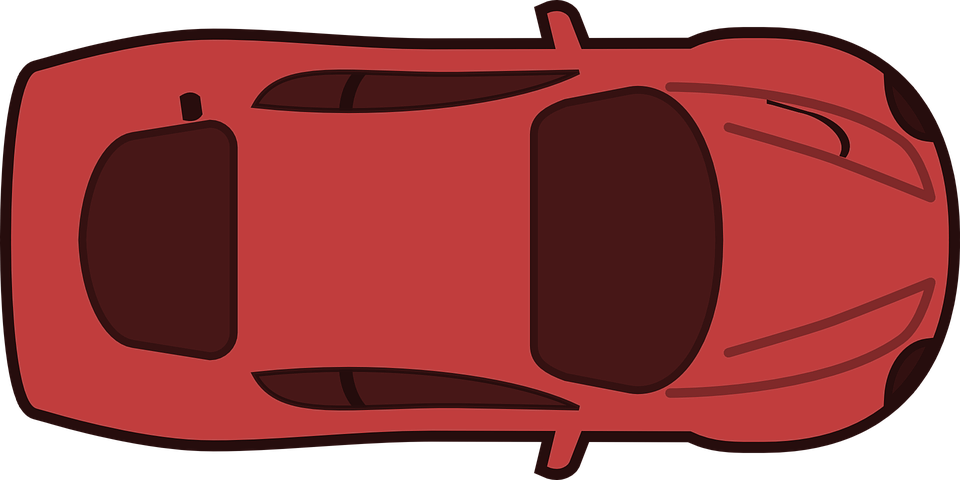
\includegraphics[width=.18\textwidth, angle=0]{figures/ego_car_top_down.png}};
			\node[inner sep=0pt] (target_car) at (0,4)
			{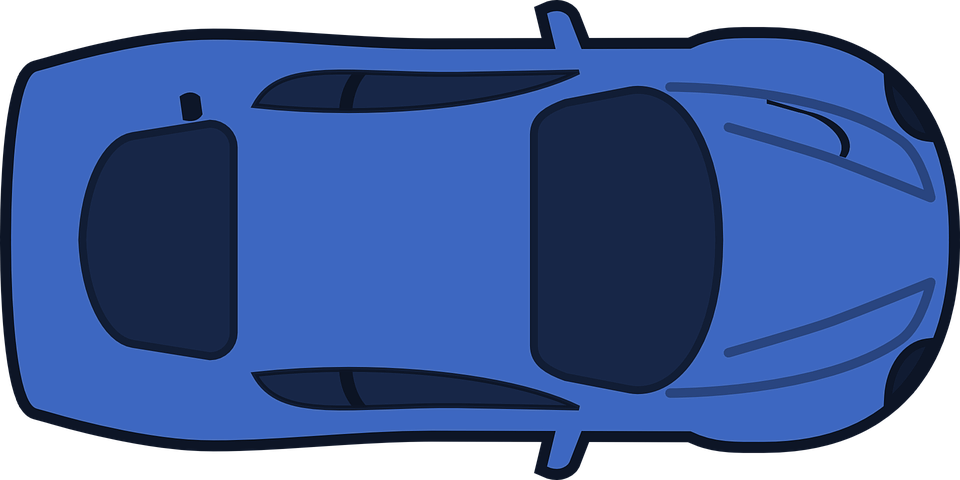
\includegraphics[width=.18\textwidth, angle=-90]{figures/target_car_top_down.png}};

	\end{tikzpicture}
	}}
	\caption{Intersection scenario divided into zones describing what is required of the decision maker in different zones}
	\label{fig:zones}
\end{figure}

With the \gls{mdp}, defined a typical intersection can be described as in Figure \ref{fig:zones}. From the figure the path of the ego vehicle can be divided into four zones. Starting from the end, zone 0 is the "safe zone" where the ego is our of danger and can return to nominal driving. Zone 1 is the conflict zone, this is where there is a possibility to collide with another vehicle. Zone 2 is critical decision zone, where this is the last chance the vehicle has to stop or cross. The size of this zone is defined as the minimal distance the car needs to come to a complete stop to the start of the conflict zone. The final zone is zone 3, the information gathering zone, and is the furthest from the intersection and where the agent can observe the scenario and the other vehicles behavior over time. 

the goal is to reach zone 0, 
to do this the agent would want to minimize the time in zone 1, if there is chance of intersection with another car.
Because our actions are formulated as options and designed to be conformtable with lower acceleration rates. The size of zone 2 is dependent on the vehicels current speed, which is dependent on how the vehicle behaved in zone 3. 
Now there are two conflicting strategies, to minimize time in zone 1 the agent wants a high speed coming into the intersection. while it would want a low speed to shorten the zone 2 and the critical decision. 

If the intention of the other vehicles is known the stochasticity in zone 1 would be gone and the problem becomes a scheduling problem of creating a velocity profile that minimizes the time to cross.  

\tommy{Deep Q-learning approach}
We want to formulate the problem in such a way that abstracts the information of traffic lights, traffic signs and intention. This way the car is closer to L5 by not relying on the different traffic lights.

One motivation example is in how traffic lights works. In Sweden, we have sensors that can sense if there are cars in an intersection and create a traffic light schedule accordingly, compared to the US where the traffic signals set up using timers. As a consequence, Drivers approaching a yellow light 

The \gls{dqn} algorithm uses a \gls{nn} and has two disadvantages. One is that the size of the network is fixed, this forces the input space to be fixed. Our state space is defined by the physical state of the surrounding cars, and the number of cars we observe at each situation variate. %Therefor we need a way to invariate of 

\section{Approach (State representation, observable and unobservable)}
This paper explored the possibility of solving the problem with \gls{rl} by trying a verity of different methods from the rainbow paper with the addition to the LSTM layer and presented the results that had the highest impact on the conversion. 
\todo{State representation}
This section describes the general state representation used in this research that enables these methods to be generalizable for different type of intersection and crossings. 
By describing the state space as a set of distances to intersection points, we can abstract the map layout of different intersections and the same algorithms would work for intersections variations that we haven't specifically trained on. 
\todo{add image of intersection scenario with 90 degree entry point and 45 degree entry point.}
\todo{Network model}
Shared weights, DQN vs DRQN. 
\todo{Learning tools}
experience replay and dropout. 
\todo{explain rewards}
large negative reward for invalid actions.
\section{Simulated experiments}
\section{Results and discussion}
\begin{itemize}
  \item STG as actions
  \item shared weights
  \item effect of replay, dropout 
  \item comparing a dqn and Drqn 
\end{itemize}
however sensitive to noise. 

LSTM take into account the history, but when applied in the real world with noise the model did not perform as well. 
The immidiate reward for jerk is 
\tommy{finding time to intersection and position itself in a way that does not conflict with other cars.}

\tommy{FIND A SECTION. Collisions in this thesis, may sound critical and extreme. But collisions in this content is for the purpose of the simulator and for the terminal state of the agent. Translated to a system perspective, it would mean that a backup collision avoidance algorithm had to interfere and in the worst case take over. }

 
\section{MPC}
\todo{rewrite}
\gls{mpc} is an optimization-based control technique where an Optimal Control Problem~(OCP) is repeatedly solved over a receding limited time horizon, starting from the current system state. In particular, for every time instance, a mathematical model of the controlled system is used to simulate the future states over a finite horizon, while a sequence of control inputs are selected and optimized given an objective cost function. The first element in the sequence of control inputs is then applied to the real system, and a new OCP with an updated state is solved at the next time instance.

\section{Approach, (Action space, options. MPC)}
\tommy{Mixed-Integer Programming (MIP) Problems
A mixed-integer programming (MIP) problem is one where some of the decision variables are constrained to be integer values (i.e. whole numbers such as -1, 0, 1, 2, etc.) at the optimal solution.  
However, integer variables make an optimization problem non-convex, and therefore far more difficult to solve.  Memory and solution time may rise exponentially as you add more integer variables.}

MPC has a mixed integer problem, calculating the optimal path for all possible action is very computationally heavy. 
RL DQN. Only has discrete actions. Can not guarantee safety but is good at choosing actions with the best utility (value). 
The reward function takes in the predicted outcome of the model in the MPC and can penalize the choice of action. but if experience show that the outcome is better than the model, it can choose to take a bad action that would lead to a better total reward compared to only following a conservative model. 

\tommy{in this work we simulate three different intention agents, take way, give way and cautious agent.}
\begin{figure}[t!]
	\mbox{\parbox{\textwidth}{
	\centering
	% \vspace{0.3cm}
	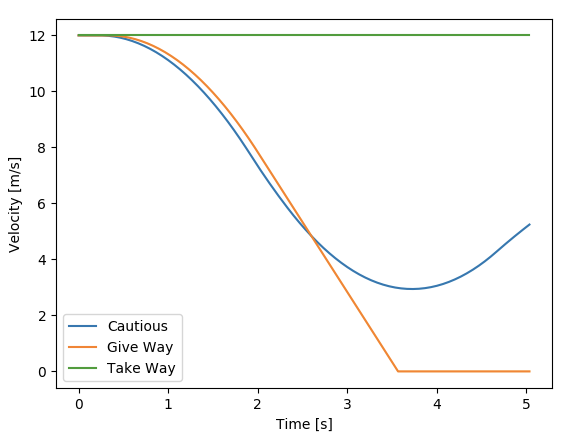
\includegraphics[width=0.7\columnwidth]{YourThesis/papers/mpc/figures/velocity_profiles_agents.png}
	}}
	\caption{Example of how velocity profile of the different intention agents can look like. All agents have the same starting velocity of $12$m/s and are approaching the same intersection}
	% \label{fig:intention_profiles}
	% \vspace{-0.3cm}
\end{figure}\
\todo{reward function}
added Q masking.
Q-masking reduce the search space, in this work we showed it for unavailable actions but could be extended to actions limited by the precautionary safety module. 
By combining the having the \gls{mpc} cost as a negative reward the \gls{dqn} can balance the control cost with the high level goal of reaching the goal and even choose an action that is on average good on a high level but may not seem that way to the \gls{mpc}.

Given the state representation, the dynamics of the vehicle is then modeled using a  triple integrator with jerk as control input.

\tommy{mpc cost function}
The objective of the agent is to safely track a reference, e.g. follow a path with a target speed, acceleration, and jerk profile, while driving comfortably and satisfying constraints that arise from physical limitations and other road users, e.g. not colliding in intersections with crossing vehicles. Hence, we formulate  the  problem as a finite horizon, constrained optimal control problem
\begin{subequations}
	\label{eq:mpc2}
	\begin{align}
	J = \min_{\bar\x,\bar\u} & \sum_{k=0}^{N-1}% \varphi_n(x_n,u_n) + \varphi_N(x_N)\\
	\matr{c}{\bar\x_k - \r_k^\x \\ \bar\u_k - \r_k^\u}^\top \matr{cc}{Q &S^\top\\S & R} \matr{c}{\bar\x_k - \r_k^\x \\ \bar\u_k - \r_k^\u} \\
	&\qquad + \matr{c}{\bar\x_N - \r_N^\x}^\top P \matr{c}{\bar\x_N - \r_N^\x}\nonumber\\
	&\text{s.t.}\ \ \, \bar\x_0 = \hat{\x}_0, \label{eq:mpcState2}\\
	&\qquad{}\bar\x_{k+1} = A\bar\x_{k}+B\bar\u_{k},\label{eq:mpcDynamics2}\\
	&\qquad{}h(\bar\x_k,\bar\u_k,\bar{\mathbf{o}}_k,a_k) \leq{} 0, \label{eq:mpcInequality2}
	\end{align}
\end{subequations}
where $k$ is  the prediction time index, $N$ is the prediction horizon, $Q$, $R$, and $S$ are the stage costs, $P$ is the terminal cost, $\bar\x_k$ and $ \bar\u_k$ are the predicted state and control inputs, $\r^\x_k$ and $\r^\u_k$ are the state and control input references, $\bar{\mathbf{o}}_k$ denotes the predicted state of vehicles in the environment which need to be avoided, and $a$ is the action from the high-level decision maker. Constraint \eqref{eq:mpcState} enforces that the prediction starts  at the current state estimate $\hat\x_0$, \eqref{eq:mpcDynamics} enforces the system dynamics, and \eqref{eq:mpcInequality} enforces constraints on the states, control inputs, and obstacle avoidance.

The reference points, $\r^\x_k$, $\r^\u_k$ are assumed to be set-points of a constant velocity trajectory, e.g. following the legal speed-limit on the road. Therefore, we set the velocity reference according to the driving limit, and the acceleration and jerk to zero.


% \tommy{Obstacle prediction}
% In order for the vehicle planner in \eqref{eq:mpc} to be able to properly avoid collisions, it is necessary to provide information about the surrounding vehicles in the environment. Therefore, similarly to \cite{batkovic2019}, we assume that a sensor system provides information about the environment, and that there exists a prediction layer which generates future motions of other vehicles in the environment. The accuracy of the prediction layer will heavily affect the performance of the planner, hence, it is necessary to have computationally inexpensive and accurate prediction methods.

% In this paper, for simplicity the future motion of other agents is estimated by a constant velocity prediction model. The motion is predicted at every time instant for prediction times $k\in[0,N]$, and is used to form the collision avoidance constraints, which we describe in the next section. Even though more accurate prediction methods do exist, e.g. \cite{lefevre2014survey,batkovic2018}, we use this simple model to show the potential of the overall framework.

% \tommy{Collision avoidance}
% % \begin{figure}[t]
% % 	\centering
% % 	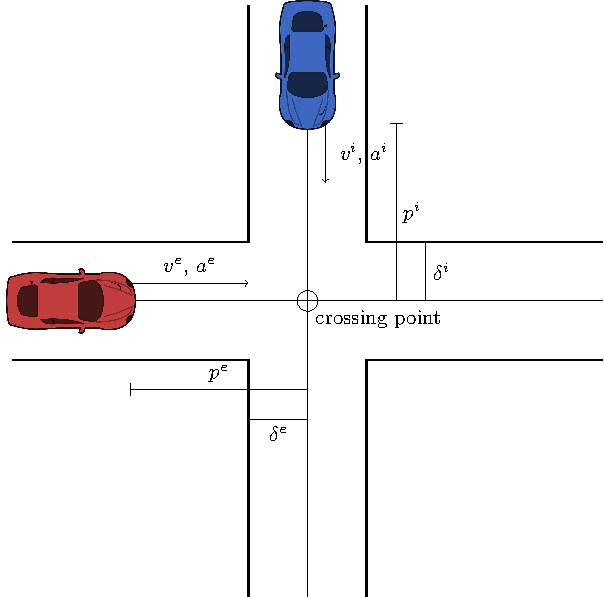
\includegraphics[width=0.6\columnwidth]{figures/figures-observations.pdf}
% % 	\caption{Observations of a scenario}
% % 	\label{fig:observations2}
% % \end{figure}\
% We denote a vehicle $j$ with the following notation $\x^j:=[p^j\, v^j\, a^j]^\top$, and an associated crossing point at position $p^{\mathrm{cross},j}$ in its own vehicle frame, which translated into the ego-vehicle frame is denoted as $p^{\mathrm{cross},j}_\mathrm{ego}$. With a predefined road topology, we assume that the vehicles will travel along the assigned paths, and that collisions may only occur at the crossing points $p^{\mathrm{cross},j}$ between an obstacle and the ego vehicle. Hence, for collision avoidance, we use the predictions of the future obstacle states $\bar\x^j_k$ for times $k\in[0,N]$, provided by a prediction layer outside of the MPC framework. Given the obstacle measurements, the prediction layer will generate future states throughout the prediction horizon. With this information, it is possible to identify the time slots when an obstacle will enter the intersection.

% Whenever an obstacle $j$ is predicted to be within a threshold of $p^{\mathrm{cross},j}$, e.g. the width of the intersecting area, the ego vehicle faces a constraint of the following form
% \begin{gather*}
% \bar{p}_k^\mathrm{e} \geq{} p^{\mathrm{cross},j}_\mathrm{ego} + \Delta,\quad\underline{p}_k^\mathrm{e} \leq{} p^{\mathrm{cross},j}_\mathrm{ego} - \Delta,
% \end{gather*}
% where $\Delta$ ensures sufficient padding from the crossing point that does not cause a collision. The choice of $\Delta$ must be at least such that $p_k$ together with the dimensions of the ego-vehicle does not overlap with the intersecting area.

% \tommy{Take way and give way constraint}
% Since the constraints from the surrounding obstacles become non-convex, we rely on the high-level policy maker to decide through action $a$ how to construct the constraint \eqref{eq:mpcInequality} for Problem \eqref{eq:mpc}. The take-way action implies that the ego-vehicle drives first through the intersection, i.e., it needs to pass the intersection before all other obstacles. This implies that for any vehicle $j$ that reaches the intersection during prediction times $k\in[0,N]$, the generated constraint needs to lower bound the state $p_k$ according to
% \begin{equation}
% \max_{j}p^{\mathrm{cross},j}+\Delta \leq{}p_k^\mathrm{e}.
% \end{equation}
% Similarly, if the action is to give way, then the position needs to be upper bounded by the closest intersection point so that
% \begin{equation}
% p_k^\mathrm{e} \leq{} \min_{j}p^{\mathrm{cross},j}_\mathrm{ego}-\Delta,
% \end{equation} 
% for all times $k$ that the obstacle is predicted to be in the intersection.

% \tommy{Following an obstacle}
% For any action $a$ that results in the following of an obstacle $j$, the ego-vehicle position is upper bounded by $p^\mathrm{e}_k \leq{} p^\mathrm{cross,j}_\mathrm{ego}$. We construct constraints for obstacles $i\neq{}j$ according to
% \begin{itemize}
% 	\item if $p^\mathrm{cross,i}<{}p^\mathrm{cross,j}$ then $p^\mathrm{cross,i}+\Delta\leq{}p_k^\mathrm{e}$, which implies that the ego-vehicle should drive ahead of all obstacles $i$ that are approaching the intersection;
% 	\item if $p^\mathrm{cross,i}>{}p^\mathrm{cross,j}$ then $p_k^\mathrm{e}\leq{}p^\mathrm{cross,i}-\Delta$, which implies that the ego-vehicle should wait to pass obstacle $j$ and other obstacles $i$;
% 	\item if $p^{\mathrm{cross,i}}=p^{\mathrm{cross},j}$ then the constraints generated for obstacle $i$ becomes an upper or lower  bound depending on if obstacle $i$ is ahead or behind the obstacle $j$ into the intersection.
% \end{itemize}


\section{Simulated experiments}
We show the difference in a multi crossing scenario where the MPC can plan a path for both intersections while our previous DQN only handles one at a time. 

\begin{figure}[t]
	\mbox{\parbox{\textwidth}{
	\centering
	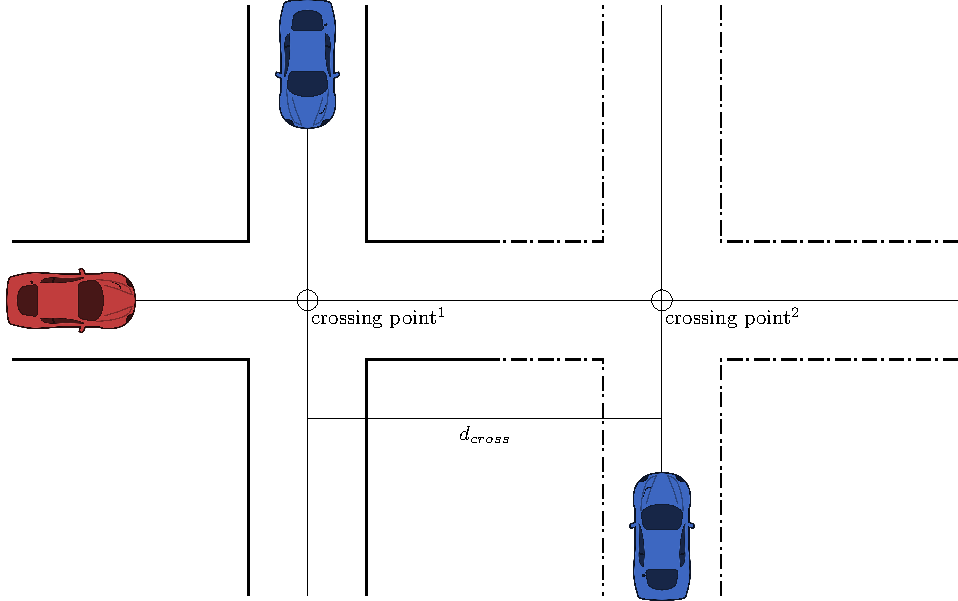
\includegraphics[width=.95\columnwidth]{YourThesis/papers/mpc/figures/figures-scenarios.pdf}
	}}
	\caption{Illustration of a intersection scenario, where the solid line is a single crossing and together with the dashed line creates a double crossing.}
	% \label{fig:scenario}
\end{figure}

\section{Results and discussion}

% \begin{figure}[t!]
	% \mbox{\parbox{\textwidth}{
% 	\centering
% 	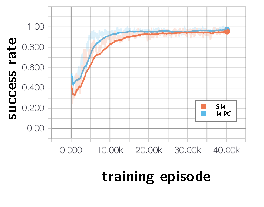
\includegraphics[width=\columnwidth]{YourThesis/papers/mpc/figures/figures-successrate.pdf}
% }}
% 	\caption{Average MPC and SM success rate for a single corssing after evaluating the policy 300 episodes.}
% 	\label{fig:result1}
% \end{figure}

% \begin{figure}[t!]
% 	\centering
% 	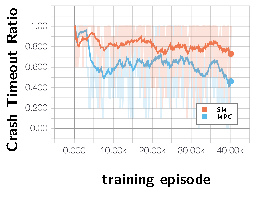
\includegraphics[width=\columnwidth]{YourThesis/papers/mpc/figures/figures-crashratio.pdf}
% 	\vspace{-4em}
% 	\caption{Average MPC and SM crash to timeout ratio for a single crossing after evaluating the policy in 300 episodes. A CTR of $0$ means that all failures are timeouts, while a CTR of $1$ means that all failures are collisions.}
% 	\label{fig:result2}
% \end{figure}

\begin{table}[t!]
	\mbox{\parbox{\textwidth}{
	\centering
	\begin{tabular}{ |p{1,6cm}||p{1,2cm}|p{1,2cm}|p{1,2cm}|p{1,2cm}|}
	\hline
	Controller &\multicolumn{2}{|c|}{Success Rate}
	&\multicolumn{2}{|c|}{Timeout Ratio}\\
	\hline
	 & Single & Double & Single & Double\\
	\hline
	SM & $96.1\%$ & $90.9\%$ & $72\%$ & $93\%$\\
	MPC & $97.3\%$ & $95.2\%$ & $45\%$ & $76\%$\\
	\hline
	\end{tabular}
	}}
	\caption{Average success rates and collision to timeout rates.}% across single and double crossings.}   

% \label{tab:successrate}
\end{table}

synergies between mpc and dqn
